\documentclass[a4paper,10pt]{scrartcl}
%encodings
\usepackage[utf8]{inputenc}
\usepackage[english]{babel}
\usepackage[T1]{fontenc}
%colors, hyperrefs
\usepackage{color}
\usepackage{url}
\usepackage[pdftex,pdfauthor={J\"org Behrmann, Anika Haller},pdftitle={Ma12: Magneto-optical Kerr-effect and Magnetic Anisotropy}]{hyperref}
%figures and subfigures
\usepackage[pdftex]{graphicx}
\usepackage{subfigure}
%better tables
\usepackage{tabularx}
\usepackage{booktabs}
\usepackage{multirow}
%math stuff
\usepackage{amsmath}
\usepackage{amsthm}
\usepackage{amsfonts}
\usepackage{IEEEtrantools}
\usepackage[square,comma,numbers,sort&compress]{natbib}
%shiny stuff
\usepackage[babel]{microtype}
\DisableLigatures{encoding=T1,family=tt*}

\begin{document}

\title{Magneto-optical Kerr-effect and Magnetic Anisotropy}
\author{J\"org Behrmann\footnote{behrmann@physik.fu-berlin.de} \qquad Anika Haller\footnote{halleran@zedat.fu-berlin.de}}
\date{31.10.2011}
\maketitle
\tableofcontents
\thispagestyle{empty}


\section{Introduction}
In this experiment we examine magnetic properties of ferromagnets and thereby are concerned with the magneto-optical Kerr effect and magnetic anisotropy.

The magneto-optical Kerr effect describes the effect of  linearly polarized light that is reflected from a magnetized media and thereby changes its polarisation by getting rotated by a certain angle. 

Magnetic anisotropy stands for the direction dependence of the magnetic properties of a material.

\subsection{Magneto-optical Kerr effect (MOKE)}


\subsection{Magnetism}
The electrons together with their spin cause a magnetic dipole moment $\mathbf{m}$. In ferromagnets, where we only have partially filled electron shells, there is a net magnetic moment. Through quantum mechanical exchange forces the magnetic moments in a ferromagnet are all aligned along one direction. This can be described by the magnetization 
\begin{eqnarray}
 \mathbf{M} = n \mathbf{m},
\end{eqnarray}
where $n$ is the number of dipoles per volume unit.

\subsection{MOKE}
The Faraday effect is the magneto-optical effect that describes light that is transmitted through magnetized matter. Moreover the Kerr effect describes light that is \textit{reflected} on a magnetized surface and thereby a change of the polarisation direction occurs. 

Together with the Lorentz force the Maxwell equations describe the fundamental electromagnetic phenomena in terms of the electric field strength $\mathbf{E}$ and the magnetic flux density $\mathbf{B}$. In the presence of matter it is convenient to formulate the macroscopic Maxwell equations with the dielectric displacement $\mathbf{D}$ and the magnetic field $\mathbf{H}$ instead of $\mathbf{E}$ and $\mathbf{B}$.
\begin{eqnarray}
 \nabla \cdot \mathbf{D}  &=& \rho_f, \\
 \nabla \times \mathbf{E} &=& -\partial_t\mathbf{B}, \\
 \nabla \cdot \mathbf{B}  &=& 0, \\
 \nabla \times \mathbf{H} &=& \mathbf{j}_f + \partial_t\mathbf{H},
\end{eqnarray}
with the free charge density $\rho_f$ and the free charge current-density $\mathbf{j}_f$.

For our experiment we are interested in the behaviour of light in anisotropic media. Therefor the dielectric displacement and the electric field strength are related through 
\begin{eqnarray}
 D_i = \varepsilon_{ij}E_j,
\end{eqnarray}
where we use  the summation convention.  The complex dielectric tensor $\mathbf{\varepsilon}$ expresses the influence of an anisotropic medium on an electromagnetic wave. In the case of linear effects we have for the magnetization $\mathbf{M}$, the dipole moment $\mathbf{p}$ and the current density $\mathbf{j}$
\begin{eqnarray}
 \mathbf{M} =  \mathbf{\chi H}, \quad \mathbf{p} = \mathbf{\alpha E}, \quad \mathbf{j} = \mathbf{\sigma E}, 
\end{eqnarray}
where $\mathbf{\chi}$ is the tensor of the magnetic susceptibility, $\mathbf{\alpha}$ is the tensor of the polarizability and $\mathbf{\sigma}$ the tensor for the specific conductivity. With the dielectric tensor 
\begin{eqnarray}
 \mathbf{\varepsilon} = \mathbf{1} + \frac{1}{\varepsilon_0}\mathbf{\alpha}- \frac{i}{\omega \varepsilon_0}\mathbf{\sigma}
\end{eqnarray}
and by using the Maxwell equations it follows
\begin{eqnarray}
 \mathbf{D} = \varepsilon_0 \mathbf{E} - i\varepsilon_0 Q \left( \mathbf{e}_M\times \mathbf{E} \right).
\end{eqnarray}
Here $Q$ is a complex constant, describing the magneto-optical coupling and $\mathbf{e}_M$ is the direction vector of the magnetization. 

Here the cross product $\mathbf{e}_M\times \mathbf{E}$ can be interpreted in a classical approach of the Kerr effect. Simplified, one can say the electrons are oscillating in the alternating electrical field. Due to the magnetization of the material, a Lorentz force affects the electrons so that the polarization of the emitted light is changed. 

There are three kinds of the MOKE, that are distinguished according to the orientation of the magnetization to the incident plane of light, which are called polar, longitudinal and transversal. 


\subsection{Magnetic anisotropy}

Magnetic anisotropy stands for the direction dependence of the magnetic properties of a material. If there is no applied magnetic field, a magnetically isotropic material has no preferred direction for its magnetic moment, whereas a magnetically anisotropic material has preferred directions for spontaneous magnetization (easy axis). This also means that there are energetic differences in different directions. 

The shape anisotropy is a result of the long range dipole-dipole interaction. It describes the stray field energy which is determined through the geometry of the magnet.

The crystal anisotropy is caused by the spin-orbit coupling where we have a coupling of the magnetic moment of an electron and the effective magnetic field that is caused by the orbital motion around the nucleus. The crystal anisotropy describes the differences of energies per volume for the spontaneous magnetization along different crystal axes. For the directions with the lowest energies we have the so called easy axes, while the other ones are called hard axes.

In the experiment we use an bcc-Fe film that is magnetized in the (100)-plane (easy axis). The crystal anisotropy can be calculated by
\begin{eqnarray}
 E_{cryst} = K_1(\cos^2{\phi}\sin^2{\phi}).
\end{eqnarray}
Here $\phi$ is the angle to the [100]-direction and $K_1$ is the first order anisotropy constant.

\subsubsection{Magnetic hysteresis}

If an external magnetic field is applied to a ferromagnetic sample an increasing  magnetization can be observed. 
When reaching the saturation magnetization all magnetic moments of the sample are aligned parallel.
After having reached the saturation magnetization, if now the external magnetic field is reduced the magnetization follows another curve. 
When the external field is zero there still is a residual magnetism, the so called remanence. Only through an oppostie directed magnetic field, the so called coercive force, the remanence disappears and the magnetization gets zero again. 
This behavior leads to the typical hysteresis curves. The reasons for this phenomena are the so called Weiss domains, which are characterized by the fact
that the electrons in these domains are parallel aligned. 

\subsection{Magnetic domains}
A ferromagnetic sample in remanence builds up a magnetic domain pattern. A domain is a region within a magnetic material where the individual magnetic moments of the atoms point in the same direction.
The magnetic domains are separated through domain walls. Within a domain wall the magnetic moments rotate from the magnetization direction of the one domain to the direction of the other domain.
 
If the rotation axis is perpendicular to the domain wall it is called a Bloch wall. 
If otherwise the rotation axis is parallel to the domain wall this one is called N\'{e}el wall. 

If an external field is applied on the magnetic domains where the moments point in the same direction with the external field become bigger, while the others get smaller. By achieving the coercive field strength the magnetization turns.

\section{Evaluation of the Experiment}

When not mentioned otherwise we use Gaussian error propagation for the calculation of errors. Fits will be made using least squares methods, either linear least squares for linear problems or Levenberg-Marquardt for nonlinear problems, implemented in \textit{Mathematica}. Errors will be given in in round brackets after a value, where a $k$-digit number gives the error in the preciding $k$ digits. 
The terms magnetic field, meaning $H=B/\mu_0$, and magnetic induction, meaning $B$, will be used interchangeably.

\subsection{Experimental Setup \label{sec:setup}}

\begin{figure}
\centering
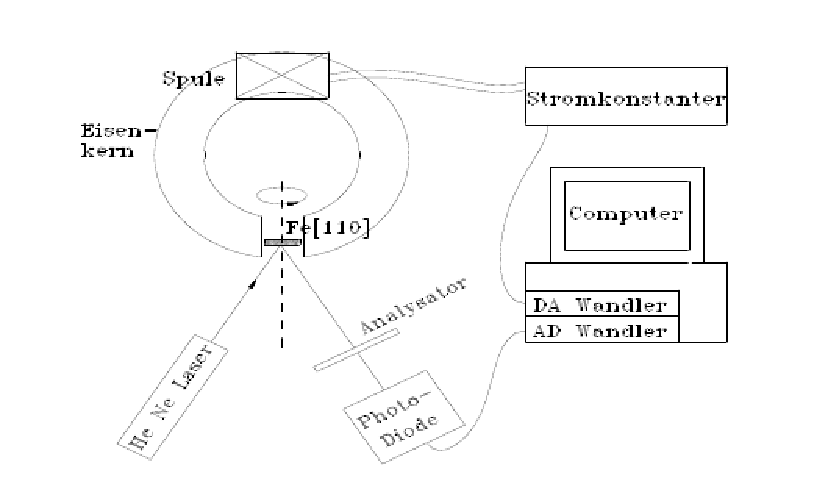
\includegraphics[scale=0.9]{img/setup}
\label{fig:setup}
\caption{Setup of the experiment taken from \cite{skript}}
\end{figure}

The experimental setup is shown in figure~\ref{fig:setup}. It consists of a HeNe-Laser producing linearly polarized light shining on a Fe-sample in a magnetic field produced by a coil with a pole shoe. The light is then reflected through an analyzer at a photodiode where the signal is measured and relayed to a computer taking the measurement data with a custom \textit{LabView} program.  For the greater part of the experiment a constant offset voltage has to be added to the signal from the photodiode, because the measurement equipment cannot resolve signal gretaer than $1.25\,$V, due to hardware restriction. The offset voltage is meaasure with a multimeter.
For the calibration task a Hall meter is used and in the setup is abadoned and a Kerr microscope is used to study a iron-garnet sample.

\subsection{Calibration of the Magnetic Field}

\subsubsection{Theoretical Expectations}

The magnetic field in solenoid, vulgo a coil, can be calculated by the use of Ampere's law, which in its integral form is given by
\begin{equation}
nI = \int_\sigma \vec{j}_f \cdot \mbox{d}\vec{a} = \int_\sigma (\nabla \times \vec{H}) \cdot \mbox{d}\vec{a} = \int_\gamma \vec{H} \cdot \mbox{d}\vec{s} = H_{Fe}s_{Fe} + H_{slit}s_{slit},
\end{equation}
where $n$ is the winding number of the coil, $I$ is the current applied to the coil, $\vec{j}_f$ is the free current density and $H$ is the magnetic field. The surface integral over $\sigma$ is transformed into a line integral by use of Stoke's theorem. The term $H_{Fe}s_{Fe}$ can be neglected compared to $H_{slit}s_{slit}$ because of the highrelative permeability of the iron core in comparisson to the air in the slit. Using the given values $n\,=\,300$ and $s_{slit}\,=\,12\,$mm the magnetic field $B\,=\,\mu_0 H$ follows as
\begin{equation}
\frac{B_{slit}}{\mu_0} = \frac{n \mu_0}{s_{slit}} = 10 \pi \mbox{mTA}^{-1} = 31.4 \mbox{mTA}^{-1}
\end{equation}

\subsection{Calibration Data}

As a preparatory task the magnetic field was calibrated using a Hall probe. The measured Hall voltage was then converted to a magnetic induction using a given conversion factor of $1\,\mbox{V}=100\,\mbox{mT}$. The measured curves, showing the hysteresis of the iron pole shoe, can be found in figure~\ref{fig:calib}. The measurements were taken once for the center of the magnetic field and once for the sample position, which for mechanical reasons is slightly off center.
To determine the right current to magnetic induction conversion factor the linear parts of the hysteresis curves between the $-2\,$A and $2\,$A were fitted with a linear model for the the upper and the lower curve each and then averaged. The calibration data can be found in table~\ref{tab:calibfits}, the constant parts of the linear fit gives a rest magnetization of the iron pole shoe at zero magnetic field, that we will not  consider further. Errors of the calibration fit are taken solely from the variance of the data and thus are only a lower bound for the error in the calibration, but we will not use them further, since the error in the applied magnetic field is neglible to all other sources of error in the following experiments. Considering only the calculated errors the calibration data does not agree with the theoretical expectations, since the theoretical expectation is several $\sigma$ away, but the agreement is sufficient for our experiment and we discarded a term in the the derivation that can further explain the disagreement to the calibration data.

\begin{figure}
\centering
\subfigure[ ]{
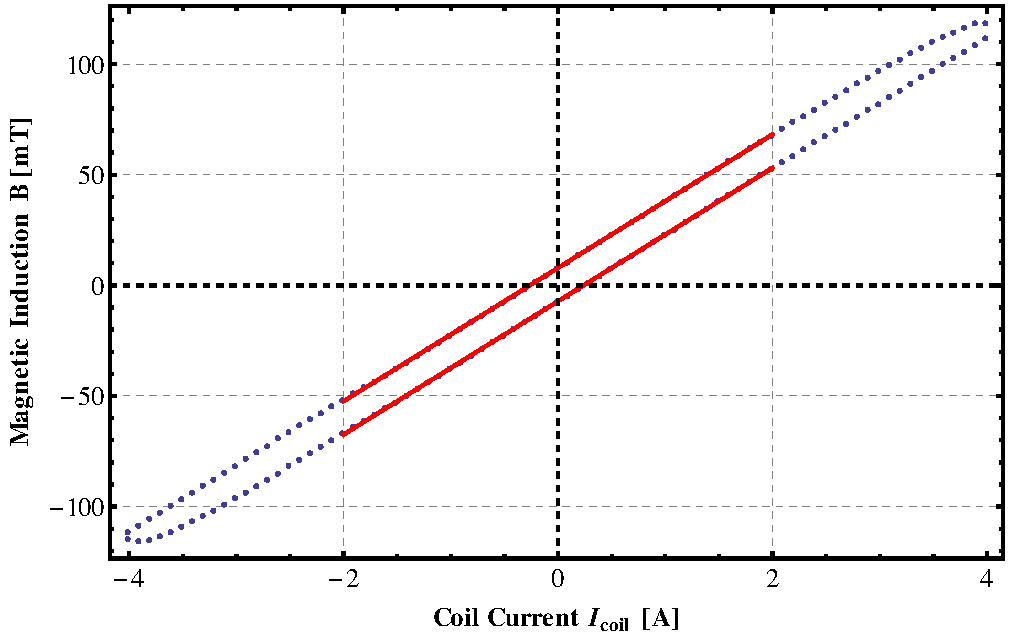
\includegraphics[scale=0.36]{img/calibborder}
\label{fig:border}
}
\subfigure[ ]{
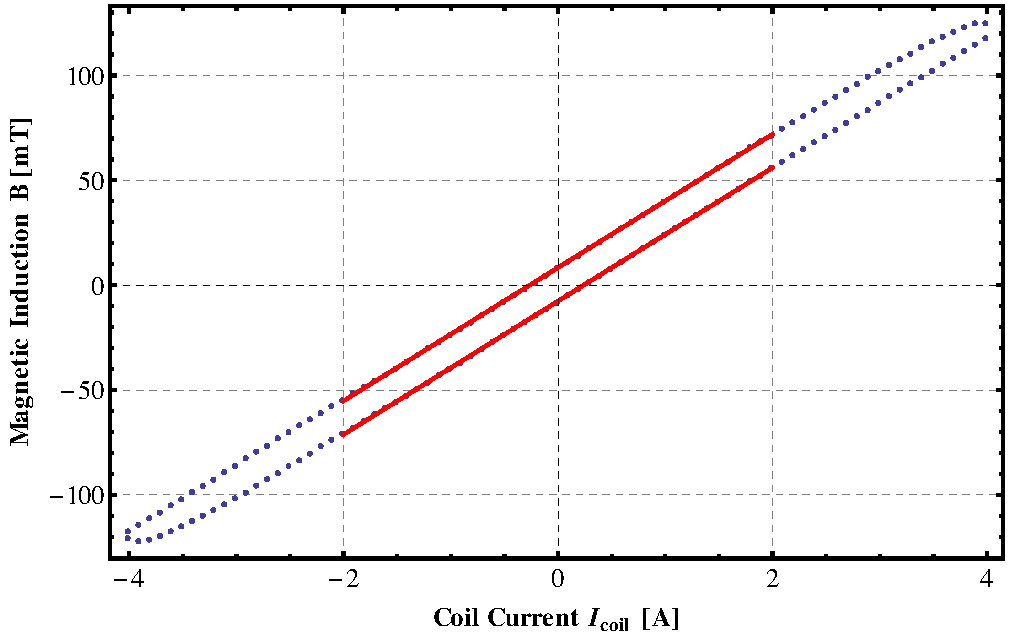
\includegraphics[scale=0.36]{img/calibcenter}
\label{fig:center}
}
\caption{Calibration curves for the border region of the magnetic field (sample position) \subref{fig:border} and the center of the magnetic field \subref{fig:center} \label{fig:calib}}
\end{figure}

\begin{table}
\begin{center}
\begin{tabular}{lcc}
\toprule
                                          & $m\,[\mbox{mT/A}]$            & $n\,[\mbox{A/m}]$ \\
\midrule
\multirow{3}{*}{Border (Sample Position)} & 30.1479(355) & \phantom{-}7.9371(409) \\
                                          & 30.1325(367) & -7.1648(424) \\
                                          & 30.014(26)\phantom{00}   & \phantom{-}0.386(30)\phantom{00}    \\
\multirow{3}{*}{Center}                   & 31.7736(377) & \phantom{-}8.4137(435) \\
                                          & 31.7985(301) & -7.5698(348) \\
                                          & 31.786(26)\phantom{00} & \phantom{-}0.422(30)\phantom{00}    \\
\bottomrule
\end{tabular}
\end{center}
\par
\caption{Fit data for the calibration curves; the first line gives the data of the upper fit, the second line gives the data of the lower fit, the third line gives the mean \label{tab:calibfits}}
\end{table}


\subsection{Determination of the Magnetic Anisotropy Constant}

In contrast to recent years~\cite{johannes} a new sample was used, making it very easy to find the [100] (easy) and [110] (hard) axis of the crystal. The hysteresis curves can be found in figure~\ref{fig:a1}. The intensitis measured at the photodiode are given in V which for the unknown conversion factor to the magnetization amounts to arbitrary units. From~\cite{skript} we know that $mu_0 M = 2.1\,T$ which could be used to rescale the plot after fitting a linear model saturation (i.e. linear) part of the [100] axis hysteresis curve and equating the mean of the absolute value of their constant parts with $2.1\,$T.

According to \cite{kittel} the anistropy energy density is given by
\begin{equation}
U_K = K_1(\alpha^{2}_{1}\alpha^{2}_{2}+\alpha^{2}_{2}\alpha^{2}_{3}+\alpha^{2}_{3}\alpha^{2}_{1}) + K_2 \alpha^{2}_{1}\alpha^{2}_{2}\alpha^{2}_{3},
\end{equation} 
which gives zero for the [100] axis, motivating the term easy, and $\tfrac{K_1}{4}$ for the [110] direction. The anisotropy energy density can be calculated as the area between the hysteresis curves in [100] and [110] direction. We calculated the area by fitting the [110] hysteresis curves linearly for the the upper left and lower parts of the curves, the upper right was fitted with two lines. The areas were then calculated by integration from the coercivity at $\pm 3.5\,$mT to the point of intersection of the fitting curves. The error for the fitting curves is determined solely by their variance, and an error of $0.5\,$mT for the coervivity was assumed. More intricate methods for computing the area under the curve could have been used, but the rescaling of the data and the accuracy of the meaasurements itself do not warrant a higher precision.  The calculated areas can be found in table~\ref{tab:a1fits}. 

The value of $K_1$ is given as $42\,$kJ/m$^3$ in~\cite{kittel} which does not agree with the mean value that can be found in table~\ref{tab:a1fits}, but agrees perfectly with the mean found from only the two lower areas. It can be argued that the upper areas can be discarded since during the measurements the current was varied from its maximally positive to the negative value and back to the positive value, which in most cases resulted in the hysteresis curve to not close properly and might also influence the upper areas in cases where they close.

\begin{figure}
\centering
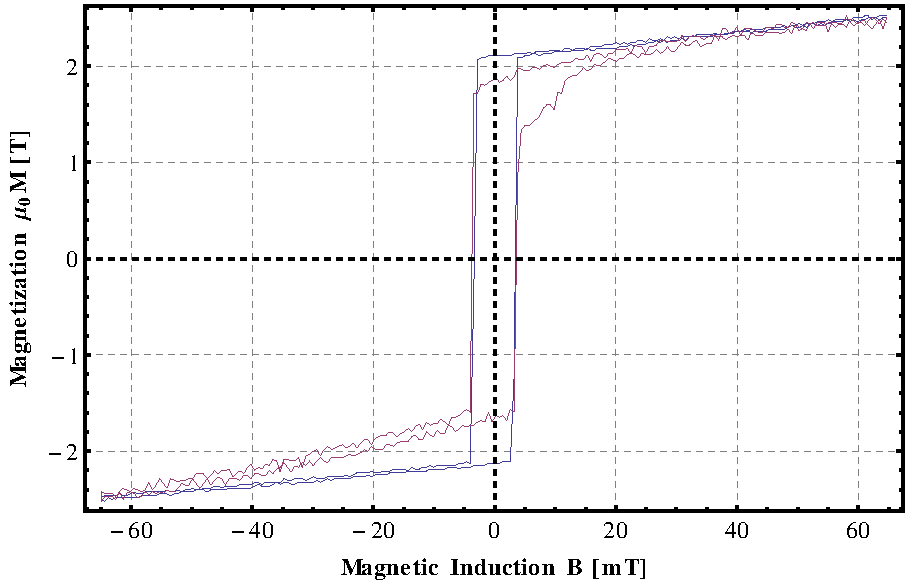
\includegraphics[scale=0.7]{img/a1}
\caption{Renormalized hysteresis curves for the [100] and [110] directions of the Fe crystal \label{fig:a1}}
\end{figure}

\begin{table}
\begin{center}
\begin{tabular}{lc}
\toprule
area       & Anisotropy Constant $K_1\,[\mbox{kJ}/\mbox{m}^3]$ \\
\midrule
a          & \phantom{0}4.65 $\pm$ 0.69 \\
b          & \phantom{0}9.8 $\pm$ 1.5 \\
c          & 13.1 $\pm$ 1.9 \\
d          & 12.2 $\pm$ 1.8 \\
mean       & 32 $\pm$ 3 \\
upper mean & 23 $\pm$ 2 \\
lower mean & 41 $\pm$ 3 \\
\bottomrule
\end{tabular}
\end{center}
\par
\caption{Anisotropy constants calculated from the uper left (a), upper right (b), lower left (c) and lower right (d) parts of the hysteresis curves and their means. \label{tab:a1fits}}
\end{table}


\subsection{Kerr Angle Measurement}

\subsubsection{Measurement equation}

The measurement equipment used in this experiment is not sensitive enough to measure the Kerr rotation directly. Fot this reason we will employ the contrast method. The contrast is defined as:
\begin{equation}
C(\alpha) = 2 \frac{I_{+}(\alpha) - I_{-}(\alpha)}{I_{+}(\alpha) + I_{-}(\alpha)}, \label{eq:contrast}
\end{equation}
where the $I_{\pm}(\alpha)$ are the maximal measured intensities at the saturation magnetizations. Equation~\eqref{eq:contrast} defines the contrast in general, but as mentioned in section~\ref{sec:setup} the equipment used can only measure voltages up to absolute values of $1.25\,$V we will have to add constant offsets to the intensities~\eqref{eq:contrast} resulting in
\begin{equation}
C(\alpha) = 2 \frac{I_{+}(\alpha) - I_{-}(\alpha)}{I_{+}(\alpha) + I_{-}(\alpha) + I_{offset}}, \label{eq:contrast2}.
\end{equation}
Furthermore it is important to note, that hysteresis curves for analyzer angles greater or smaller than the angle of minimal intensity will have different directions. While going from the lower left to the upper right for angles greater than the angle of minimal intensity, as can be seen in figure~\ref{fig:a1}, they will go from the upper left to the lower right for angles smaller than the angle of minimal. This is important because the nomenclature $I_{\pm}$ is bit misleading, implying that this are the maximal and minimal intensities and although they are the intensities with the greatest absolute value, discarding the small linear growth in apparent saturation, they should be rather seen as the intensities of greatest absolute value when coming following the hysteresis curves either from left or right. This means that the contrast will have a a different sign when measured for analyzer angles greater or smaller than the angle of minimal intensity.

Since the measured intensities are that of linearly polarized after passing an analyzer, thus the intensities are given by Malus's law
\begin{equation}
I(\alpha) = I_0 \cos^{2}(\alpha), \label{eq:malus}
\end{equation} 
obviously having its maximum intensity at $\alpha = 0$. For convenience we will measure the contrast around the point of minimal intensity. Furthermore we cannot expect the intensity to drop to zero for two reasons. Firtly \eqref{eq:malus} only holds for perfect analyzers, secondly the Kerr effect not only rotates the polarization of the incoming light, but also makes it slightly elliptical. We will therefore use
\begin{equation}
I_{\pm}(\alpha) = I_0 \sin^{2}\left((\alpha - \alpha_{0}) + \phi_{K}\right) + I_{Rest}, \label{eq:malus2}.
\end{equation} 
Inserting the above equation in \eqref{eq:contrast} and expanding the sines for small angles, we arrive at the measurement equation
\begin{equation}
C(\alpha) = \frac{4 (\alpha - \alpha_0) \phi_K}{(\alpha - \alpha_0)^2 + \phi^{2}_{K} + \frac{I_{Rest}}{I_0}}. \label{eq:measure}
\end{equation}
The $\phi^{2}_{K}$ in the denominator can be neglected since the Kerr angle will be very small, but we chose not to, since it did not make a difference for the complexity of the fits, we made.

\subsection{Determination of Kerr Angle \label{sec:kerrangle}}

To determine the Kerr angle we first search for the the angle of minmal intensity by coarsely rotating the analyzer, which we found roughly between $125.5$ and $126\,$degrees. We then took hysteresis curves around that angle in half degree steps. We took three angles to the left angle of angle of minimal intensity and eleven to the right of it, one of those was taken at $126.25\,$degrees. As mentioned earlier the offset voltage had to be adjusted multiple times to take the measurements. Due to time restrictions the measurements were only taken for s-polarized light.

From the measured intensities the contrast data was calculated. From equation~\eqref{eq:contrast2} we can see that the contrast consists of the intensities read off from the hysteresis curves, for which we assume an error of $0.03\,$V, and the offset for which we assumed an error of $0.5\,$\%$+1\,$digit. We then plotted the contrast and the inverse contrast and fitted the measurement equation~\eqref{eq:measure} in different forms, as seen in table~\ref{tab:a2fits}. This was done because some of the forms converged better to the data than others, which also varied for different subsets of the data and starting values for the fitting algorithm. The three points to the left of the angle of minimal intensity never fittet well in any fit and their inclusion only decreased the accordance with the points to the right of the angle of minimal intensity. 

Some exemplary plots of the fits can be found in figure~\ref{fig:kerrfit}.  The fit data is shown in table~\ref{tab:a2fits} and is consistent for each choice of data subset. By taking the mean we can infer the Kerr angle to be at approximately $\phi_K = -0.03\,$degrees, but unfortunately the different data subsets remain incompatible, because of the very small errors that were calculated for the fitting parameters by including the contrast errors as weights in the fits. The small value of the Kerr angle fits our expectation and justfies the approximations made earlier a posteriori.

Whereas the Kerr angles are at least in the approximate vicinity of each other for the different subsets, the ratios of minimal intensity $I_{Rest}$ to $I_0$ remain utterly incompatible. This points to a flaw in our experimental data and would constitute a reason the take new measurements, more equally distributed on both sides of the angle of minimal intensity, which was not done in our original experiment due to time restrictions. We would argue therefore neglect the three leftmost points, because they do not fit the points on the right and are too few to be fitted with any of our models by itself conclusively.

\begin{table}
\begin{center}
\begin{tabular}{lccc}
\toprule
Model                                                                                                                                                           & $\alpha_{0}\,[\mbox{deg}]$ & $\phi_{K}\,[\mbox{deg}]$ & $\tfrac{I_{Rest}}{I_{0}}\,[1]$ \\
\midrule
\multirow{2}{*}{$C = \frac{4 \alpha \phi_{K}}{(\alpha - \alpha_{0})^2 + \phi^{2}_{K} + \frac{I_{Rest}}{I_{0}}}$}                                                            & 125.90(3) & -0.0297(4) & 1.50(8) \\
                                                                                                                                                                            & 125.80(5) & -0.0317(6) & 2.1(8)\phantom{0}  \\ 
\multirow{2}{*}{$C = \frac{1}{\frac{1}{4 \phi_K} (\alpha - \alpha_{0}) + \left(\frac{\phi_K}{4} + \frac{I_{Rest}}{4 \phi_K I_0}\right)\frac{1}{(\alpha - \alpha_{0})}}$}    & 125.90(3) & -0.0297(4) & 1.50(7) \\
                                                                                                                                                                            & 125.80(5) & -0.032(3)\phantom{0}  & 2.1(2)\phantom{0}  \\
\multirow{2}{*}{$\frac{1}{C} = \frac{1}{4 \phi_K} (\alpha - \alpha_{0}) + \left( \frac{\phi_L}{4} + \frac{I_{Rest}}{4 \phi_K I_0} \right) \frac{1}{(\alpha - \alpha_{0})}$} & 125.80(3) & -0.0296(6) & 1.10(5) \\
                                                                                                                                                                            & 125.75(7) & -0.0321(7) & 2.2(2)\phantom{0}  \\
                                                                                                                                                                            & 124(7)    & -0.04(2)\phantom{00}   & ---     \\
\bottomrule
\end{tabular}
\end{center}
\par
\caption{Fit data for Contrast plots, fitted with different models. The first line of a row gives the fit for all data points, the second line was only fitted to the data points with angles greater than the angle of minimal intensity. The last line gives the fit for the linear part of the inverse contrast. \label{tab:a2fits}}
\end{table}

\begin{figure}
\centering
\subfigure[ ]{
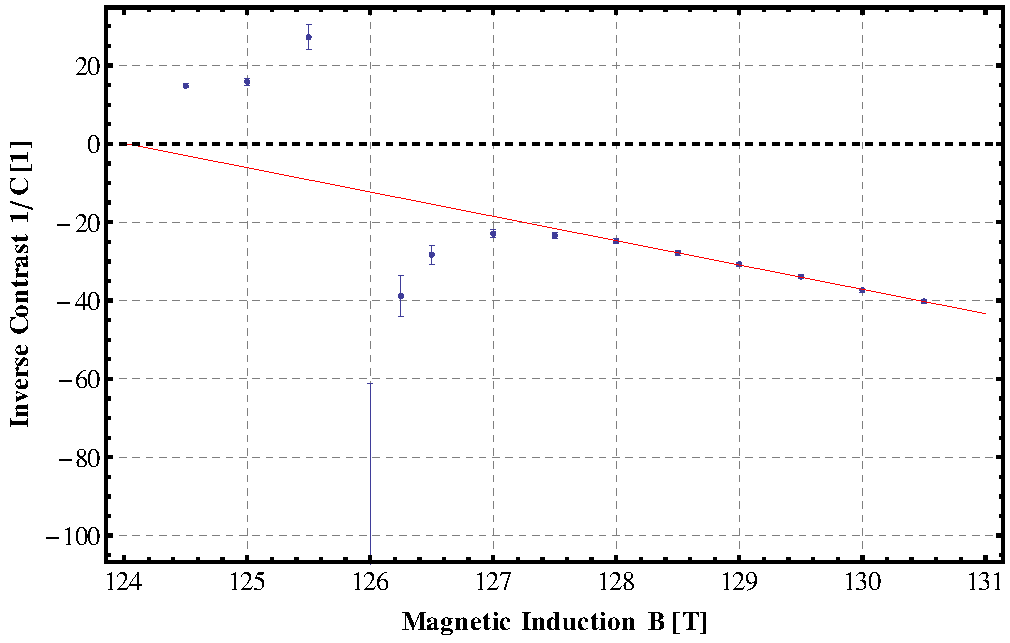
\includegraphics[scale=0.36]{img/a2invlin}
\label{fig:a2invlin}
}
\subfigure[ ]{
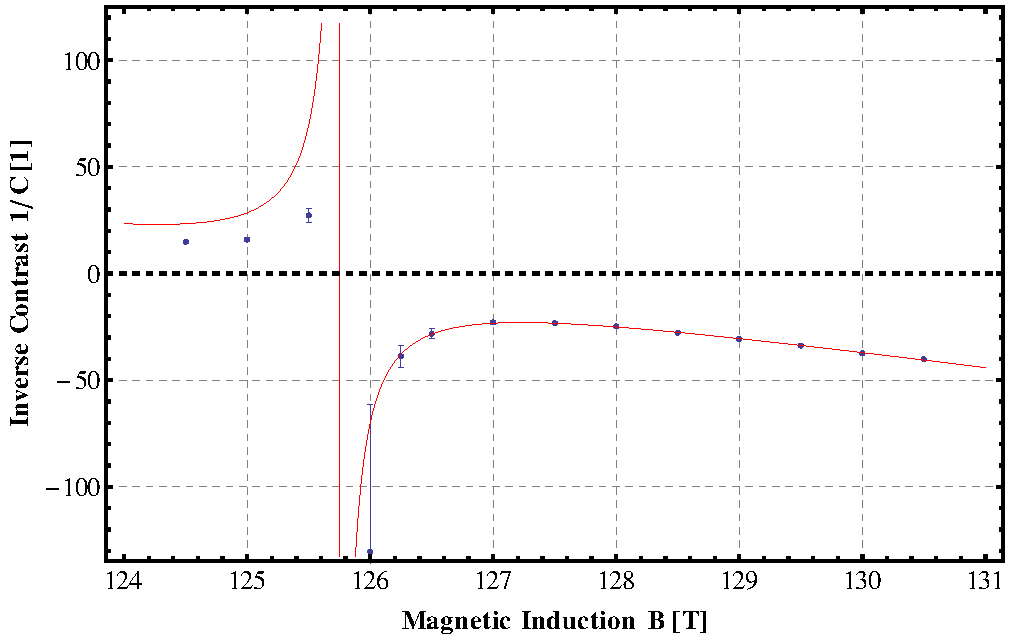
\includegraphics[scale=0.36]{img/a2inv}
\label{fig:a2inv}
}
\subfigure[ ]{
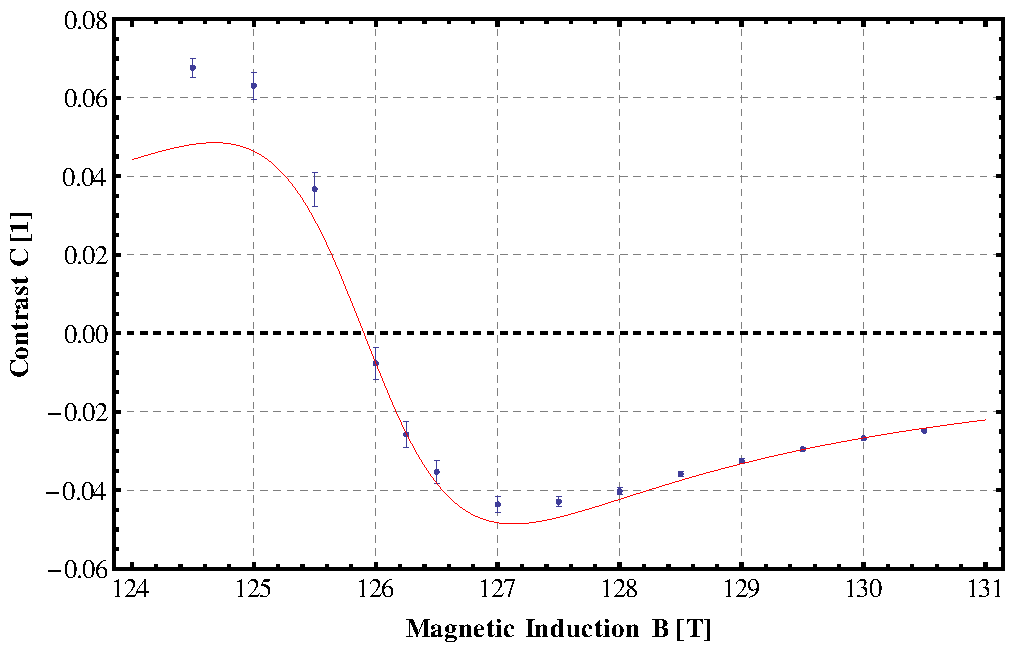
\includegraphics[scale=0.36]{img/a2all}
\label{fig:a2all}
}
\subfigure[ ]{
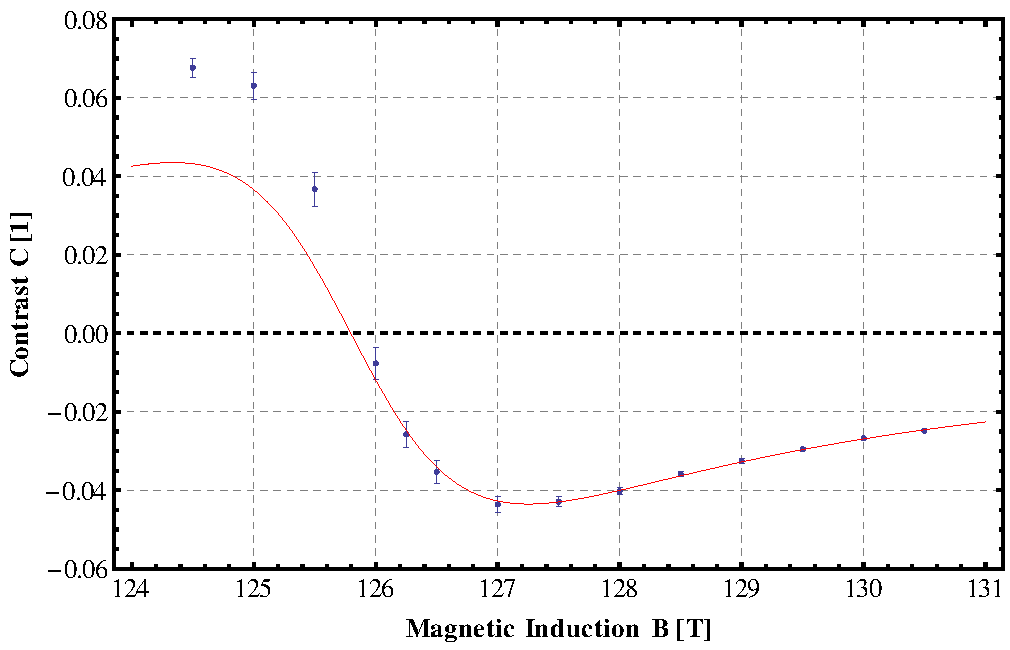
\includegraphics[scale=0.36]{img/a2}
\label{fig:a2}
}
\caption{Contrast fits for the linear part of inverse contrast \subref{fig:a2invlin}, inverse contrast \subref{fig:a2inv} (three leftmost points excluded), the contrast including all points \subref{fig:a2all} and \subref{fig:a2} with the three leftmost points excluded \label{fig:kerrfit}}
\end{figure}

\subsection{Dependence of the Kerr Angle on the Angle of Incidence}

For this task the position of the arm, on which the analyzer and the photodiode rested, was varied to vary the angle between of incidence of the light on the Fe-sample and measure a theoretically expected dependence of the Kerr angle on the angle of incidence. We did this for incidence angles between $20$ and $45\,$degrees in $5\,$degree steps for s-polarized light and, due to time restrictions, $10\,$degree steps for p-polarized light. The lower bound of $20\,$degrees is due to mechanical reasons, because the arms could not be brought any nearer to each to other.

For each angle of incidence a hysteresis curve was measured and the contrast calculated as in~\ref{sec:kerrangle}. It is most important to realize that the usual assumptions of errorless independent variables does not hold for this task, because the angle of incidence carries an error that is not neglible to the measurement errors, because it is at least of the same order of magnitude, if not bigger as in the case of p-polarized light. This can be seen in figure~\ref{fig:angledep}, which also contain the cosine fits expeted from~\cite{zak}. Nonlinear fits for models with in-variable-errors are non-trivial and are not worth for this qualitative problem, which is why we only fitted the contrast data with the measurement errors as weights. This is enough to verify the angle of incidence-dependence of the Kerr angle, which can be seen by the very good fit. The very good fit was to be expected because of the small variation in the contrast and the very large errors. Without more data basically everything could be into this data points, which was seen during evaluation on the many parameter sets that fitted the data, which verifies the dependence on the angle of incidence but makes any quantification of it impossible.

\begin{figure}
\centering
\subfigure[ ]{
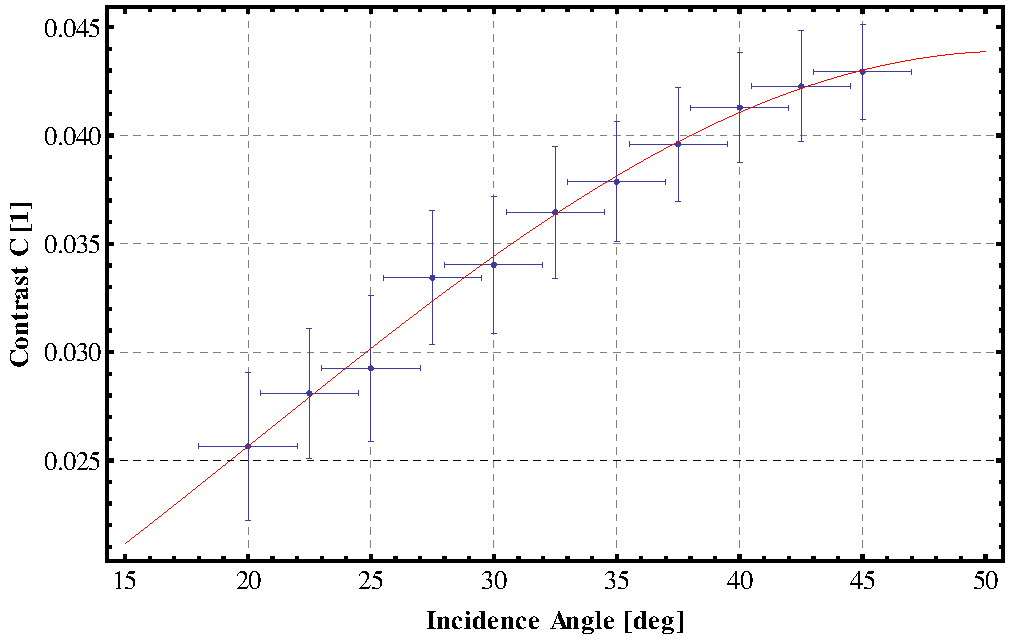
\includegraphics[scale=0.36]{img/a3s}
\label{fig:a3s}
}
\subfigure[ ]{
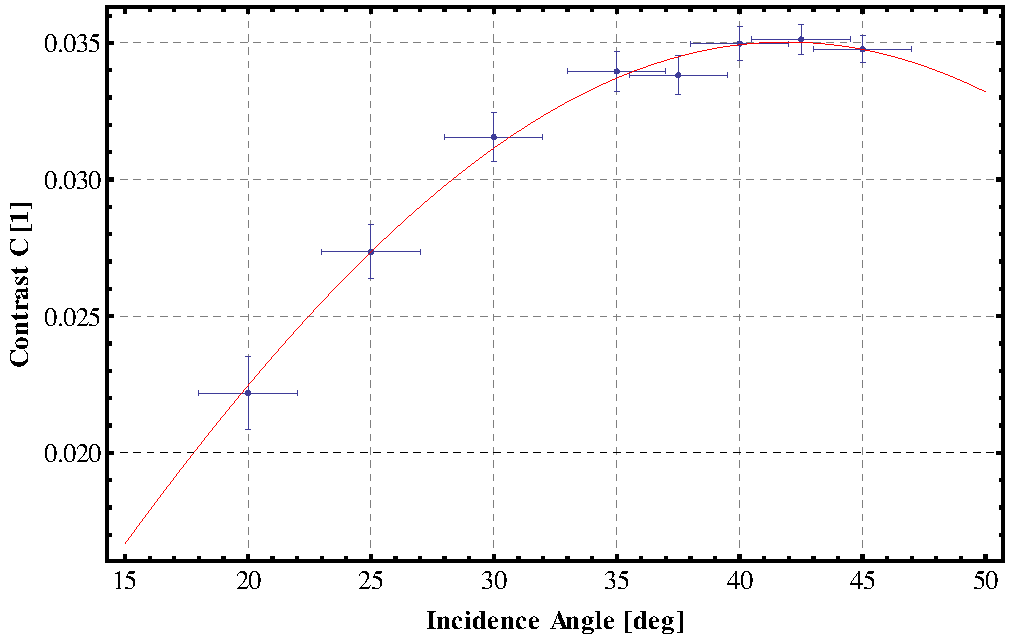
\includegraphics[scale=0.36]{img/a3p}
\label{fig:a3p}
}
\caption{Contrast fits as a function of incidence angle for s-polarized light \subref{fig:a3s} and p-polarized light \subref{fig:a3p} \label{fig:angledep}}
\end{figure}

\subsection{Kerr Microscopy}

In this task an iron-garnet was observed with a Kerr microscope. The Kerr microscope's magnetic field is highly anisotropic, thus the magnetization will be in the plane of the film. Under this circumstances, the iron-garnet is a material that exhibits Bloch domain walls. 

To compare the size of the domain walls a several year old hair of Prof. Dr. Katharina Franke is included in all pictures. The figures~\ref{fig:domainpos} and \ref{fig:domainneg} show a state with many domains at positive and negative polarity of the magnet. The picture was improved by substracting a picture of the appropriate one domain state from the pictures, then increasing the contrast and brightness of the picture, mapping a Gaussian filter on the picture and reimproving the contrast and brightness again. 

Although the picture for the negative polarity is not as good as the on for the positive polarity, can we see that inverting the polarity of the magnetic field inverts the color of the domains and domain walls.

Figures~\ref{fig:evo3} to \ref{fig:evo1} show the evolution of domains when applying an increasingly greater magnetic field from a state with many to a state with fewer domains.

To estimate the size of a domain wall we rasterized figure~\ref{fig:domainpos} and estimated the width  of the hair with about $135\pm5\,$Pixels and width fo the domain wall to about $8\pm2\,$Pixels, the larger error estimate for the hair is because it is not directly in the focus of the microscope.  According to~\cite{blume} a blinde caucasian hair is $40$ to $80\,\mu$m in diameter, thus we will use a value of $(60\pm 20)\,\mu$m. Using the ratio obtained from our estimated pixel widths we can calculate the width of the domain wall to be $(4\pm 1)\,\mu$m. This seems realistic~\cite{wiki}.

\begin{figure}
\centering
\subfigure[ ]{
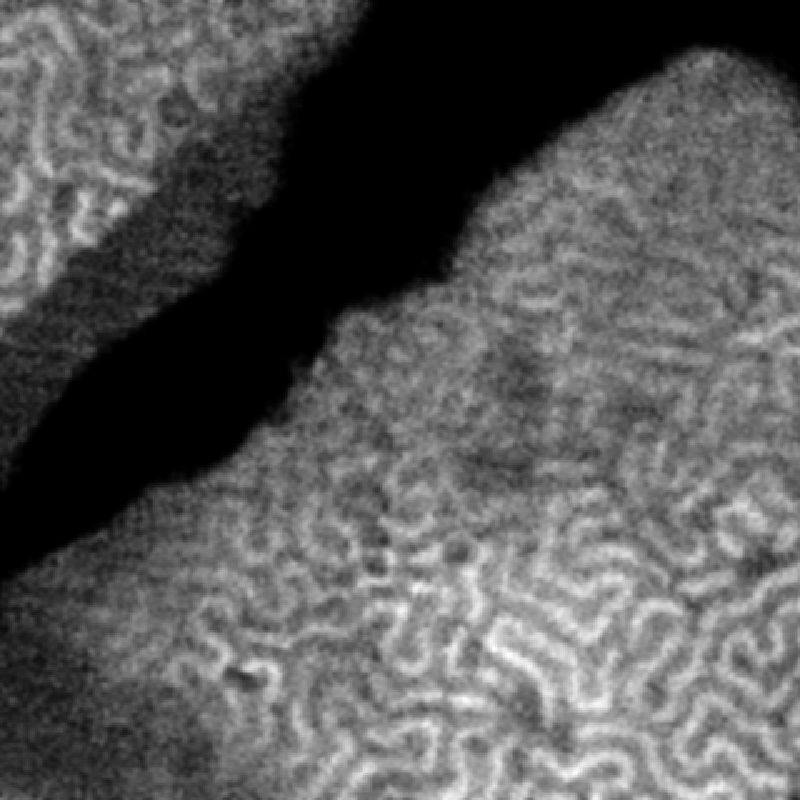
\includegraphics[scale=0.46]{img/domains1}
\label{fig:domainpos}
}
\subfigure[ ]{
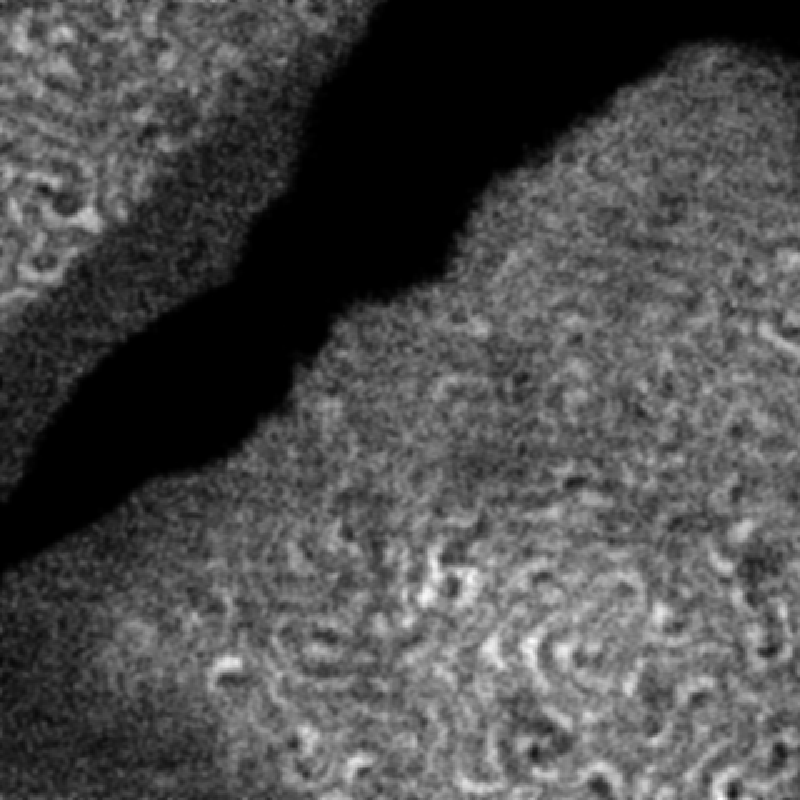
\includegraphics[scale=0.46]{img/domains2}
\label{fig:domainneg}
}
\subfigure[ ]{
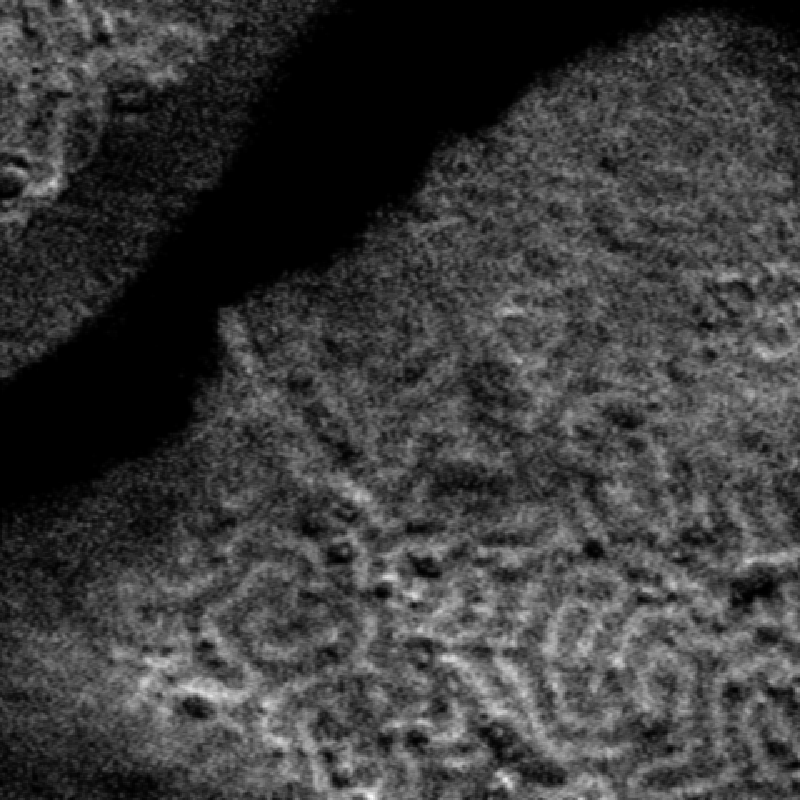
\includegraphics[scale=0.3]{img/evo3}
\label{fig:evo3}
}
\subfigure[ ]{
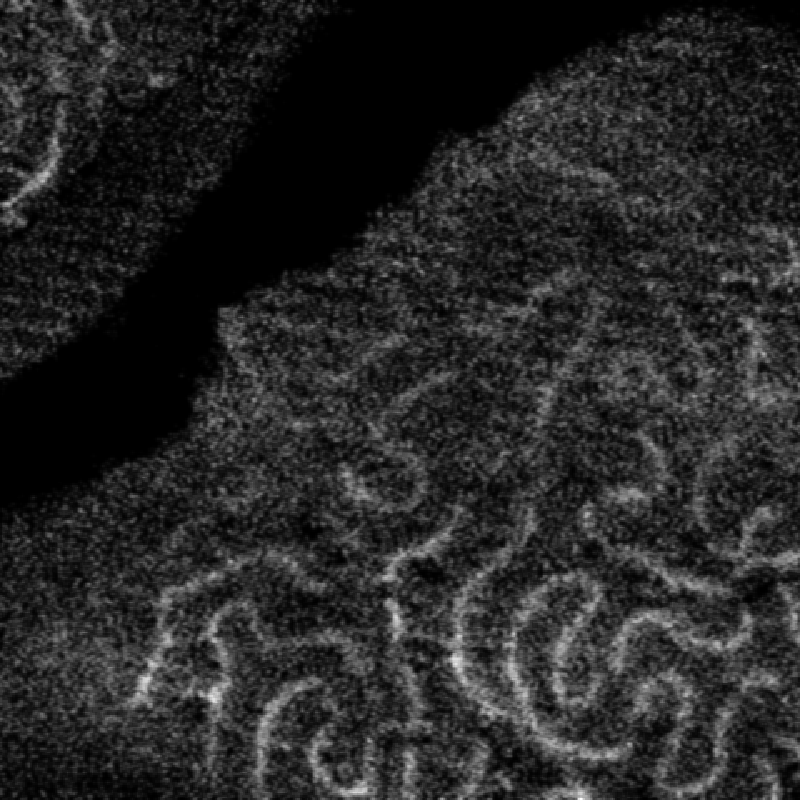
\includegraphics[scale=0.3]{img/evo2}
\label{fig:evo2}
}
\subfigure[ ]{
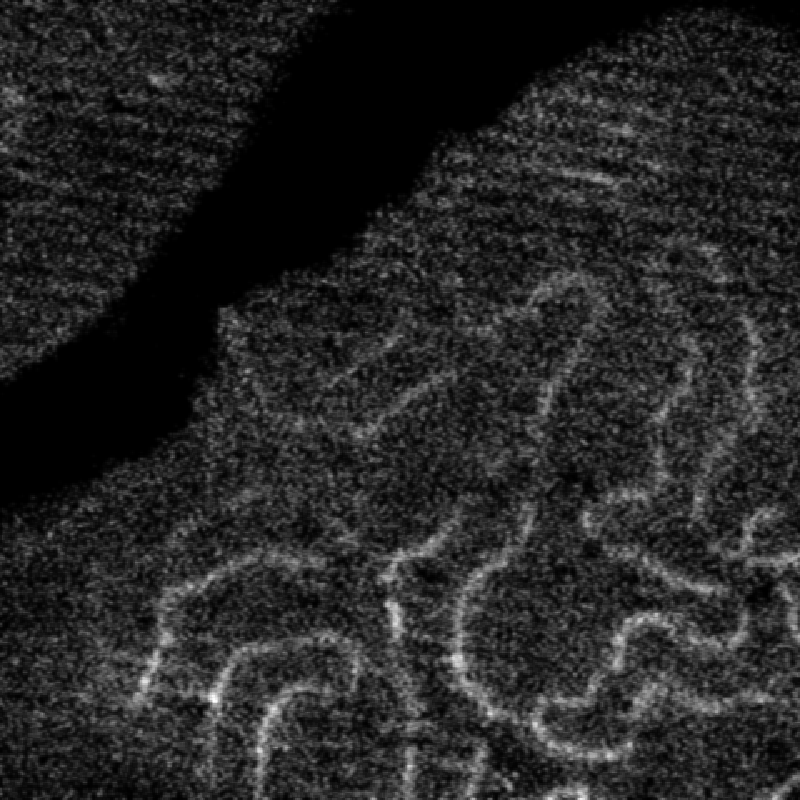
\includegraphics[scale=0.3]{img/evo1}
\label{fig:evo1}
}
\caption{Domains for positive \subref{fig:domainpos} and negative \subref{fig:domainneg} polarity of the magnet and evolution of the domains wall from a many-domains \subref{fig:evo3} to a one-domain \subref{fig:evo1} state}
\end{figure}

\section{Conclusions}

We analyzed the Magneto-optic Kerr effect in a Fe-sample and identified the easy and hard axis of magnetization. We calculated and discussed the value of the obtained anisotropy constant $K_1$, that fits the expected value very well, when some part of the data is omitted.

The Kerr rotation angle was measured using the contrast method, but differing values in the intensity ratio point to flaws in our fits and would need more data to be discused properly. Furthermore the dependence of the Kerr angle on the angle of incidence of the light was qualitatively verified using the same technique.

Finally an iron-garnet film was examined with a Kerr microscope. The images were improved using image processing techniques. The contrast inversion when chaning the polraity of the magnetic field and the evolution of the domain walls when applying magnetic fields at different strength was observed. We also gave a rough estimate for the domain wall width.

\nocite{skript}
\nocite{griffiths}
\nocite{kittel}
\nocite{meyer}
\nocite{zak}
\nocite{blume}
\nocite{wiki}
\nocite{johannes}


\bibliographystyle{plainnat}
\bibliography{kerr}

\end{document}
